\documentclass[10pt]{beamer}
\usepackage[utf8]{inputenc}
\usepackage[T1]{fontenc}
\usetheme{metropolis}
\usepackage{booktabs}
\usepackage[scale=2]{ccicons}
\usepackage{pgfplots}
\usepgfplotslibrary{dateplot}
\usepackage{xspace}
\usepackage{pbox}
\usepackage[normalem]{ulem}
\usepackage{soul}

% graphics path
\graphicspath{{./images/}}

% a few macros
\newcommand{\bi}{\begin{itemize}}
\newcommand{\ei}{\end{itemize}}
\newcommand{\ig}{\includegraphics}
\newcommand{\x}{\color{red}{$\times$}}
\definecolor{hilight}{RGB}{235,129,27}
\definecolor{vhilight}{RGB}{235,129,27}
\newcommand{\colr}[1]{\color{red}{#1}}

% title info
\title{Teoría de números}
\author{Miguel Ortiz}
\institute{Octubre 2023}
\date{\textbf{Programación competitiva para ICPC}}

% Tikz
\usepackage{tikz}
\usetikzlibrary{arrows,shapes}

% Minted
\usepackage{minted}
\usemintedstyle{manni}
\newminted{cpp}{fontsize=\footnotesize}

% Graph styles
\tikzstyle{vertex}=[circle,fill=black!50,minimum size=15pt,inner sep=0pt, font=\small]
\tikzstyle{selected vertex} = [vertex, fill=red!24]
\tikzstyle{edge} = [draw,thick,-]
\tikzstyle{dedge} = [draw,thick,->]
\tikzstyle{weight} = [font=\scriptsize,pos=0.5]
\tikzstyle{selected edge} = [draw,line width=2pt,-,red!50]
\tikzstyle{ignored edge} = [draw,line width=5pt,-,black!20]
\tikzstyle{vertex1} = [vertex, fill=red]
\tikzstyle{vertex2} = [vertex, fill=blue]
\tikzstyle{vertex3} = [vertex, fill=green, text=black]
\tikzstyle{vertex4} = [vertex, fill=yellow, text=black]
\tikzstyle{vertex5} = [vertex, fill=pink, text=black]
\tikzstyle{vertex6} = [vertex, fill=purple]

\tikzset{
  treenode/.style = {align=center, inner sep=0pt, text centered,
    font=\sffamily},
  vertex/.style = {treenode, circle, black, font=\sffamily\bfseries\tiny, draw=black, text width=1.8em},% arbre rouge noir, noeud noir
  rvertex/.style = {treenode, circle, black, font=\sffamily\bfseries\tiny, draw=red, text width=1.8em},% arbre rouge noir, noeud noir
}


\begin{document}
\maketitle

\begin{frame}
  \begin{center}
    ¿Cuál es la menor potencia de 2 que es divisible entre 3?
    
    \vspace{20pt}

    \onslide<2-> Pregunta trampa
  \end{center}
\end{frame}

\begin{frame}{Introducción}
  \bi
    \item Es un área de las matemáticas que estudia las propiedades de los números enteros
    \item Los números primos son muy importantes para su análisis
    
    \vspace{20pt}

    \item<2-> Se dice que un número es primo si es un número natural mayor a 1 y no es representable como el producto de dos naturales menores a él
    \item<2-> Solo tiene dos divisores: 1 y él mismo
    \item<3-> Los números no primos se llaman \textit{compuestos}
  \ei
\end{frame}

\begin{frame}[fragile]{Encontrar divisores}
  \bi
    \item Se puede iterar por todos los números entre 1 y $n$ y verificar si el residuo de la división es 0
  \ei
  \begin{minted}{cpp}
    for (int i = 1; i <= n; i++) {
      if (n % i == 0) {
        // i es divisor de n
      }
    }
  \end{minted}
  \bi
    \item $O(n)$
  \ei
\end{frame}

\begin{frame}[fragile]{Encontrar divisores}
  \bi
    \item Si $d$ divide a $n$, entonces $\frac{n}{d}$ también divide a $n$
    \item Si revisamos todos los valores $d$ tal que $d \leq \frac{n}{d}$, solo necesitamos iterar hasta $\sqrt{n}$
  \ei
  \begin{minted}{cpp}
    for (int i = 1; i*i <= n; i++) {
      if (n % i == 0) {
        // i es divisor de n
        // n/i es divisor de n
      }
    }
  \end{minted}
  \bi
    \item $O(\sqrt{n})$
    \item<2-> Podemos usar esto para verificar si un número es primo
  \ei
\end{frame}

\begin{frame}{Criba de Eratóstenes}
  \bi
    \item Es posible encontrar todos los primos de $1$ a $n$ en $O(n \sqrt{n})$ con el anterior método
    \item La criba de Eratóstenes encuentra todos los primos de $1$ a $n$ en $O(n \log \log n)$
    
    \vspace{20pt}

    \item<2-> El algoritmo construye un arreglo \mintinline{cpp}|criba| marcando todos los números compuestos
    \bi
      \item<2-> \mintinline{cpp}|criba[i]| es \mintinline{cpp}|true| si $i$ es compuesto
      \item<2-> \mintinline{cpp}|criba[i]| es \mintinline{cpp}|false| si $i$ es primo
    \ei
    \item<3-> Se revisan los números de $2$ a $n$, si el número es primo, se marcan todos sus múltiplos como compuestos
  \ei
\end{frame}

\begin{frame}[fragile]{Criba de Eratóstenes}
  \begin{minted}{cpp}
    vector<bool> criba(n+1, false);
    criba[0] = criba[1] = true; // 0 y 1 no son primos
    for (int i = 2; i <= n; i++) {
      if (!criba[i]) {
        // i es primo
        for (int j = 2*i; j <= n; j += i) {
          criba[j] = true;
        }
      }
    }
  \end{minted}

  \vspace{10pt}

  \begin{center}
    \begin{overprint}
      \onslide<1>\begin{tabular}{cccccccccccccccccccc}
        \colr{1} & \color{teal}{2} & 3 & 4 & 5 & 6 & 7 & 8 & 9 & 10 & 11 & 12 & 13 & 14 & 15 \\
        \hline
        16 & 17 & 18 & 19 & 20 & 21 & 22 & 23 & 24 & 25 & 26 & 27 & 28 & 29 & 30 \\
      \end{tabular}
      \onslide<2>\begin{tabular}{cccccccccccccccccccc}
        \colr{1} & \color{teal}{2} & 3 & \colr{4} & 5 & \colr{6} & 7 & \colr{8} & 9 & \colr{10} & 11 & \colr{12} & 13 & \colr{14} & 15 \\
        \hline
        \colr{16} & 17 & \colr{18} & 19 & \colr{20} & 21 & \colr{22} & 23 & \colr{24} & 25 & \colr{26} & 27 & \colr{28} & 29 & \colr{30} \\
      \end{tabular}
      \onslide<3>\begin{tabular}{cccccccccccccccccccc}
        \colr{1} & \color{teal}{2} & \color{teal}{3} & \colr{4} & 5 & \colr{6} & 7 & \colr{8} & 9 & \colr{10} & 11 & \colr{12} & 13 & \colr{14} & 15 \\
        \hline
        \colr{16} & 17 & \colr{18} & 19 & \colr{20} & 21 & \colr{22} & 23 & \colr{24} & 25 & \colr{26} & 27 & \colr{28} & 29 & \colr{30} \\
      \end{tabular}
      \onslide<4>\begin{tabular}{cccccccccccccccccccc}
        \colr{1} & \color{teal}{2} & \color{teal}{3} & \colr{4} & 5 & \colr{6} & 7 & \colr{8} & \colr{9} & \colr{10} & 11 & \colr{12} & 13 & \colr{14} & \colr{15} \\
        \hline
        \colr{16} & 17 & \colr{18} & 19 & \colr{20} & \colr{21} & \colr{22} & 23 & \colr{24} & 25 & \colr{26} & \colr{27} & \colr{28} & 29 & \colr{30} \\
      \end{tabular}
      \onslide<5>\begin{tabular}{cccccccccccccccccccc}
        \colr{1} & \color{teal}{2} & \color{teal}{3} & \colr{4} & \color{teal}{5} & \colr{6} & 7 & \colr{8} & \colr{9} & \colr{10} & 11 & \colr{12} & 13 & \colr{14} & \colr{15} \\
        \hline
        \colr{16} & 17 & \colr{18} & 19 & \colr{20} & \colr{21} & \colr{22} & 23 & \colr{24} & 25 & \colr{26} & \colr{27} & \colr{28} & 29 & \colr{30} \\
      \end{tabular}
      \onslide<6>\begin{tabular}{cccccccccccccccccccc}
        \colr{1} & \color{teal}{2} & \color{teal}{3} & \colr{4} & \color{teal}{5} & \colr{6} & 7 & \colr{8} & \colr{9} & \colr{10} & 11 & \colr{12} & 13 & \colr{14} & \colr{15} \\
        \hline
        \colr{16} & 17 & \colr{18} & 19 & \colr{20} & \colr{21} & \colr{22} & 23 & \colr{24} & \colr{25} & \colr{26} & \colr{27} & \colr{28} & 29 & \colr{30} \\
      \end{tabular}
      \onslide<7>\begin{tabular}{cccccccccccccccccccc}
        \colr{1} & \color{teal}{2} & \color{teal}{3} & \colr{4} & \color{teal}{5} & \colr{6} & \color{teal}{7} & \colr{8} & \colr{9} & \colr{10} & \color{teal}{11} & \colr{12} & \color{teal}{13} & \colr{14} & \colr{15} \\
        \hline
        \colr{16} & \color{teal}{17} & \colr{18} & \color{teal}{19} & \colr{20} & \colr{21} & \colr{22} & \color{teal}{23} & \colr{24} & \colr{25} & \colr{26} & \colr{27} & \colr{28} & \color{teal}{29} & \colr{30} \\
      \end{tabular}
    \end{overprint}
  \end{center}
\end{frame}

\begin{frame}[fragile]{Encontrar factores primos}
  \bi
    \item Queremos encontrar los factores primos de un número $x$
    \item Guardamos los primos en un vector mientras realizamos la criba
    \item El exponente de $p$ es igual a la cantidad de veces que $p$ divide a $x$
  \ei
  \begin{minted}{cpp}
    map<int, int> factorizacion;
    for (int p : primos) if (x % p == 0) {
      int e = 0;
      while (x % p == 0) {
        x /= p;
        e++;
      }
      factorizacion[p] = e;
    }
    if (x > 1) factorizacion[x] = 1;
  \end{minted}
  \bi
    \item<2-> Si generamos la criba hasta $n$, funciona para $x \leq n^2$ en $O(\pi(n))$
  \ei
\end{frame}

\begin{frame}[fragile]{Encontrar factores primos}
  \begin{minted}{cpp}
    vector<bool> criba(n+1, false);
    vector<int> primoMasGrande(n+1, -1);
    criba[0] = criba[1] = true; // 0 y 1 no son primos
    for (int i = 2; i <= n; i++) {
      if (!criba[i]) {
        // i es primo
        for (int j = 2*i; j <= n; j += i) {
          criba[j] = true;
          primoMasGrande[j] = i;
        }
      }
    }
  \end{minted}
  \bi
    \item<2-> Ya no tenemos que buscar los primos en el vector \mintinline{cpp}|primos|
    \item<2-> Con una criba hasta $n$, acelera lo anterior a $O(\log n)$ para $x \leq n$
  \ei
\end{frame}

\begin{frame}{Teorema fundamental de la aritmética}
  \begin{center}
    Todo entero mayor a 1 puede ser representado como un \textbf{único} producto de números primos
    
    \vspace{10pt}

    $n = p_1^{n_1} p_2^{n_2} \cdots p_k^{n_k} = \prod_{i=1}^{k}p_i^{n_i}$
  \end{center}

  \vspace{20pt}

  \onslide<2->{Por ejemplo:}
  \onslide<2->\bi
    \item $999 = 2^3 \cdot 37$
    \item $1000 = 2^3 \cdot 5^3$
    \item $1001 = 7 \cdot 11 \cdot 13$
  \ei
\end{frame}

\begin{frame}{GCD y LCM}
  \bi
    \item Greatest Common Divisor (Máximo Común Divisor)
    \bi
      \item Dados dos números $a$ y $b$, su GCD es el mayor número que divide a ambos
    \ei
    \item Least Common Multiple (Mínimo Común Múltiplo)
    \bi
      \item Dados dos números $a$ y $b$, su LCM es el menor número que es múltiplo de ambos
    \ei
  \ei
\end{frame}

\begin{frame}{GCD y LCM}
  \bi
    \item Podemos calcular el GCD y LCM de dos números usando sus factorizaciones

    \item $p^a \cdot p^b = p^{a+b}$
    \item $p^a / p^b = p^{a - b}$

    \item<2-> Si $d$ es un divisor de $n$, $n$ debe tener todos los primos de $d$ en su factorización con un exponente mayor o igual
    \item<3-> $\gcd(a, b)$ es el número cuya factorización tiene los exponentes mínimos entre $a$ y $b$ por cada primo
    \item<3-> Similarmente, $\text{lcm}(a, b)$ tiene los exponentes máximos
    \vspace{10pt}
    \item<4-> $\gcd(2^3 \cdot 3^2 \cdot 5^1, 2^2 \cdot 3^4 \cdot 7^1) = 2^2 \cdot 3^2$
    \item<5-> $\text{lcm}(2^3 \cdot 3^2 \cdot 5^1, 2^2 \cdot 3^4 \cdot 7^1) = 2^3 \cdot 3^4 \cdot 5^1 \cdot 7^1$
  \ei
\end{frame}

\begin{frame}[fragile]{GCD y LCM}
  \bi
    \item Este método es bueno para pensar en soluciones o demostrarlas, pero no es eficiente y es tedioso de implementar
    \item Se pueden usar las funciones ya presentes en los lenguajes para calcular el GCD y LCM
  \ei
  \onslide<2->\begin{minted}{cpp}
    __gcd(a, b)
  \end{minted}
  \onslide<3->\bi
    \item Para calcular el LCM, podemos usar la fórmula $\text{lcm}(a, b) = \frac{a \cdot b}{\gcd(a, b)}$
  \ei
\end{frame}

% TODO: Problema de ejemplo con GCD o LCM

\section{Aritmética modular}

\begin{frame}{Aritmética modular}
  \bi
    \item Recordemos que $\frac{a}{m} \rightarrow a = m \cdot c + r$, siendo $c$ el cociente y $r$ el residuo
    \item La aritmética modular trabaja solo con los residuos
    \item $a \mod m \rightarrow$ residuo de dividir $a$ entre $m$
  \ei
\end{frame}

\begin{frame}{Aritmética modular}
  \bi
    \item Es útil visualizar los residuos como posiciones en un reloj de tamaño $m$
    \item Observemos lo que pasa aumentando valores de 1 en 1 con división entre 3
    \bi
      \item $0 / 3 = 0 \text{ reciduo } 0$
      \item $1 / 3 = 0 \text{ reciduo } 1$
      \item $2 / 3 = 0 \text{ reciduo } 2$
      \item $3 / 3 = 1 \text{ reciduo } 0$
      \item $4 / 3 = 1 \text{ reciduo } 1$
      \item $5 / 3 = 1 \text{ reciduo } 2$
      \item $6 / 3 = 2 \text{ reciduo } 0$
    \ei
    \item<2-> Los residuos aumentan de 1 en 1 hasta llegar al módulo menos 1, luego vuelven a 0 y se repiten
    \item<3-> Empezar en la posición 0 del reloj y avanzar $x$ posiciones es equivalente a calcular $x \mod m$
  \ei
\end{frame}

\begin{frame}{Aritmética modular}
  $8 \mod 4 = 0$
  
  \begin{center}
    \ig[height = 0.5\textheight]{8mod4.jpg}
  \end{center}
\end{frame}

\begin{frame}{Aritmética modular}
  $7 \mod 2 = 1$
  
  \begin{center}
    \ig[height = 0.5\textheight]{7mod2.jpg}
  \end{center}
\end{frame}

\begin{frame}{Aritmética modular}
  $-5 \mod 3 = 1$
  
  \begin{center}
    \ig[height = 0.5\textheight]{-5mod3.jpg}
  \end{center}
\end{frame}

\begin{frame}{Operaciones}
  \bi
    \item \textbf{Congruencia}: $a \equiv b \mod m \longrightarrow a \mod m = b \mod m$
  \ei
\end{frame}

\begin{frame}[fragile]{Operaciones}
  \bi
    \item Veremos las siguientes operaciones como se harían en un lenguaje de programación
  \ei
  \begin{minted}{cpp}
    int r = a % m;
  \end{minted}
  \bi
    \item<2-> \textbf{Suma}: $(a + b) \% m = (a \% m + b \% m) \% m$, avanzar en el reloj
    \item<3-> \textbf{Resta}: $(a - b) \% m = (a \% m - b \% m + m) \% m$, cuidado con negativos
  \ei
\end{frame}

\begin{frame}{Operaciones}
  \bi
    \item \textbf{Multiplicación}: $(a \cdot b) \% m = (a \% m \cdot b \% m) \% m$
    \item<2-> ¿Por qué?
    \item<3-> Desarrollando:
    \onslide<4->\begin{enumerate}
      \item<4-> $((m \cdot c_a + r_a) \cdot (m \cdot c_b + r_b)) \% m$
      \item<5-> $(m^2 \cdot c_a \cdot c_b + m \cdot c_a \cdot r_b + m \cdot c_b \cdot r_a + r_a \cdot r_b) \% m$
      \\ \onslide<6->{Repartimos el módulo en la suma}
      \item<6-> $((m^2 \cdot c_a \cdot c_b \% m) + (m \cdot c_a \cdot r_b \% m) + (m \cdot c_b \cdot r_a \% m) + (r_a \cdot r_b \% m)) \% m$
      \item<7-> $(0 + 0 + 0 + (r_a \cdot r_b \% m)) \% m$
      \item<8-> $r_x = x \% m \rightarrow (a \% m \cdot b \% m) \% m$
    \end{enumerate}
  \ei
\end{frame}

\begin{frame}{Operaciones}
  \bi
    \item \textbf{División}: $(a / b) \% m = (a \% m \cdot b^{-1} \% m) \% m$
    \item No podemos repartir en la división
    \item Ej: $\frac{21}{7} \mod 5 \neq \frac{21\mod 5}{7\mod 5} = \frac{1}{2}$
    
    \vspace{20pt}

    \item<2-> $a^{-1} \mod m$ es el inverso modular de $a$ módulo $m$
    \item<2-> ¿Cómo obtenemos $a^{-1} \mod m$?
    \item<3-> Pequeño teorema de Fermat: $a^{m - 1} \equiv 1 \mod m$, si $m$ es primo y $a$ no es múltiplo de $m$
    \item<4-> $a^{m - 2} \equiv a^{-1} \mod m$
    \item<5-> $(a / b) \% m = (a \% m \cdot b^{m-2} \% m) \% m$
  \ei
\end{frame}

\begin{frame}{Operaciones}
  \begin{center}
    \begin{tabular}{lcl}
      $(a + b) \% m$     & $=$ & $(a \% m + b \% m) \% m$ \\[10pt]
      $(a - b) \% m$     & $=$ & $(a \% m - b \% m + m) \% m$ \\[10pt]
      $(a \cdot b) \% m$ & $=$ & $(a \% m \cdot b \% m) \% m$ \\[10pt]
      $(a / b) \% m$     & $=$ & $(a \% m \cdot b^{m-2} \% m) \% m$ \\
    \end{tabular}
  \end{center}
\end{frame}

\begin{frame}{Potenciación binaria}
  \bi
    \item Para calcular $b^{m-2} \mod m$, necesitamos una forma eficiente de calcular potencias
    \item Multiplicar $b$ $m$ veces es $O(m)$, $m$ suele ser un valor cercano a $10^9$
    \item<2-> La función \mintinline{cpp}|pow(b, e)| de C++ encuentra una aproximación, problemas de precisión
  \ei
\end{frame}

\begin{frame}{Potenciación binaria}
  \bi
    \item $b^e = b \cdot b \cdot b \cdots b \cdot b \cdot b$
    \item<2-> Si $e$ es par $\rightarrow b^e = b^{e/2} \cdot b^{e/2}$
    \item<3-> Si $e$ es impar $\rightarrow b^e = b^{e-1} \cdot b$
    \item<4-> Seguimos reduciendo $e$ hasta llegar a $b^0 = 1$ o $b^1 = b$
  \ei
\end{frame}

\begin{frame}{Potenciación binaria}
  \begin{figure}
    \begin{tikzpicture}[scale=1.8,auto,swap]
        \onslide<1->{\node[vertex] (0) at (0.5,3) {$2^6$};}
        \onslide<2->{\node[vertex] (1) at (0,2) {$2^3$};}
        \onslide<2->{\node[vertex] (2) at (1,2) {$2^3$};}
        \onslide<3->{\node[vertex] (3) at (-0.5,1) {$2^2$};}
        \onslide<3->{\node[vertex] (4) at (0.5,1) {$2$};}
        \onslide<4->{\node[vertex] (5) at (-1,0) {$2$};}
        \onslide<4->{\node[vertex] (6) at (0,0) {$2$};}

        \onslide<2->{\path[edge] (0) -- (1); \path[edge] (0) -- (2);}
        \onslide<3->{\path[edge] (1) -- (3); \path[edge] (1) -- (4);}
        \onslide<4->{\path[edge] (3) -- (5); \path[edge] (3) -- (6);}

        \only<2-6>{\node[vertex,fill=vhilight] (0) at (0) {$2^6$};}
        \only<3-5>{\node[vertex,fill=vhilight] (1) at (1) {$2^3$};}
        \only<4>{\node[vertex,fill=vhilight] (3) at (3) {$2^2$};}
        \only<5->{
          \node[vertex,fill=green] (3) at (3) {$4$};
          \node[vertex,fill=green] (5) at (5) {$2$};
          \node[vertex,fill=green] (6) at (6) {$2$};
        }
        \only<6->{
          \node[vertex,fill=green] (1) at (1) {$8$};
          \node[vertex,fill=yellow] (2) at (2) {$2^3$};
          \node[vertex,fill=green] (4) at (4) {$2$};
        }
        \only<7->{
          \node[vertex,fill=green] (0) at (0) {$64$};
          \node[vertex,fill=green] (2) at (2) {$8$};
        }
        
        \pgfresetboundingbox
        \path [use as bounding box] (0,0) rectangle (1,3.2);
    \end{tikzpicture}
  \end{figure}
\end{frame}

\begin{frame}[fragile]{Potenciación binaria}
  \begin{minted}{cpp}
    int binPow(int b, int e, int mod) {
      if (e == 0) return 1;
      if (e == 1) return b;
      int res;
      if (e % 2 == 0) {
        res = binPow(b, e / 2);
        res = res * res % mod;
      } 
      else {
        res = binPow(b, e - 1) * b % mod;
      }
      return res;
    }
  \end{minted}
\end{frame}

\end{document}
